\documentclass[11pt,a4paper]{article}
\usepackage[margin=2.1cm]{geometry}
\usepackage{fontspec}
\usepackage{booktabs,graphicx,amsmath,array,caption,float,xcolor}
\usepackage[hidelinks]{hyperref}
\TeXXeTstate=1
\newfontfamily\dev{Noto Sans Devanagari}[Script=Devanagari,Scale=0.92]
\newfontfamily\guj{Noto Sans Gujarati}[Script=Gujarati,Scale=0.92]
\newfontfamily\gur{Noto Sans Gurmukhi}[Script=Gurmukhi,Scale=0.92]
\newfontfamily\tam{Noto Sans Tamil}[Script=Tamil,Scale=0.85]
\newfontfamily\tel{Noto Sans Telugu}[Script=Telugu,Scale=0.92]
\newfontfamily\urd{Noto Naskh Arabic}[Script=Arabic,Scale=1.0]
\setlength{\parskip}{4pt}\setlength{\parindent}{0pt}
\captionsetup{font=small,labelfont=bf}
\title{\textbf{FOVL Assignment: Multilingual Word Embeddings for Indian Languages}\\[2pt]\large Experimental Report}
\author{Aishwarya Mishra \quad USN / Roll No.: G25AIT2137\\ PG Diploma in AI, IIT Jodhpur}
\date{13 November 2026}
\begin{document}
\maketitle
\vspace{-6pt}
\begin{abstract}
I train 300-dimensional word embeddings from scratch on the IndicCorpV2-5k corpus and evaluate them on the word-similarity benchmark of Akhtar et al.\ (2017) for Gujarati, Hindi, Marathi, Punjabi, Tamil, Telugu and Urdu. The final model is a single FastText skip-gram model with character 3--6-grams, trained on the 35{,}000 documents of the seven benchmark languages (1.69M tokens). Out-of-vocabulary (OOV) words are composed from their character n-grams, so no word pair is discarded. The model reaches a macro-average Spearman correlation of $\rho = 0.240$ on the public benchmark, from 0.174 (Telugu) to 0.333 (Gujarati). Twelve experiments compare it with a count-based PPMI-SVD baseline (best $\rho = 0.179$), CBOW, skip-gram without subwords, fewer epochs, and training on all 24 corpus languages.
\end{abstract}

\section{Introduction}
Word embeddings map words to dense vectors whose geometry reflects distributional similarity. For Indian languages two properties make this hard. The languages are morphologically rich: Tamil and Telugu are agglutinative, and Hindi, Marathi and Gujarati inflect nouns and verbs heavily, so many surface forms are rare or unseen. They are also written in six different scripts (Devanagari, Gujarati, Gurmukhi, Tamil, Telugu, Perso-Arabic). The assignment adds a third constraint: only a 5{,}000-document-per-language subset of IndicCorpV2 may be used, so the models see roughly 0.2--0.4M tokens per language, orders of magnitude less than typical embedding corpora.

The goal is a model that (i) produces exactly 300-dimensional vectors, (ii) gives a meaningful vector for any input word, including OOV words, and (iii) maximises the macro-average Spearman correlation with human similarity judgements across the seven benchmark languages. This report describes the method (Section~2), visualises the learned space (Section~3), reports results and coverage (Section~4), the experiments behind the design choices (Section~5), a qualitative error analysis (Section~6), and design choices and limitations (Section~7).

\section{Methodology}
\subsection{Data}
\textbf{Training corpus.} The only training data is \texttt{rony000013/indiccorpV2-5k} (one file, \texttt{data.parquet}, 118{,}243 documents, columns \texttt{language}, \texttt{code}, \texttt{text}): 5{,}000 documents for each of 24 languages (Kashmiri: 3{,}243). The final model is trained on the seven benchmark languages only (Table~1); Experiment~E8 shows that adding the other 17 languages did not help. Because the seven languages use six scripts, one joint model is in practice close to seven monolingual models that share a parameter matrix. The exception is Hindi and Marathi, which share Devanagari n-grams and many loanwords.

\textbf{Benchmark.} The word-similarity files of Akhtar et al.\ (2017) are used only for evaluation. Files are tab-separated except Hindi (comma-separated). The public Marathi file has 253 pairs, but only the first 104 carry a human score. All 253 pairs are embedded and exported, and $\rho$ is computed on the 104 scored ones. In total, 1102 pairs are exported and 952 are scored.
\begin{table}[H]\centering\small
\caption{IndicCorpV2-5k statistics after preprocessing (tokens = maximal runs of Unicode letters, marks and digits).}
\begin{tabular}{lrrr}\toprule
Language & Documents & Tokens & Types \\\midrule
Gujarati & 5,000 & 206,598 & 39,714 \\
Hindi & 5,000 & 286,864 & 25,761 \\
Marathi & 5,000 & 208,329 & 45,849 \\
Punjabi & 5,000 & 275,660 & 27,017 \\
Tamil & 5,000 & 172,479 & 55,821 \\
Telugu & 5,000 & 174,853 & 45,710 \\
Urdu & 5,000 & 362,382 & 31,065 \\
\midrule
Other 17 languages & 83,243 & 2,806,131 & -- \\
\bottomrule\end{tabular}\end{table}

\subsection{Preprocessing}
The same normalisation is applied to corpus text and benchmark words: Unicode NFC normalisation, removal of format characters (category Cf: zero-width joiner/non-joiner, BOM), and lower-casing (which only affects Latin script). Tokens are maximal runs of Unicode letters, combining marks and digits (\verb|[\p{L}\p{M}\p{N}]+|). Keeping marks inside tokens is essential, because Indic vowel signs and viramas are combining marks. Punctuation, including the danda ({\dev ।}, {\dev ॥}) and Urdu marks ({\urd ۔}, {\urd ،}), is removed. Documents with fewer than two tokens are dropped. No stemming, transliteration or stop-word removal is applied, so morphology is left to the subword model.

\subsection{Model}
I use FastText (Bojanowski et al., 2017), as implemented in gensim 4.4.0. Each word $w$ is represented by its own vector $\mathbf{z}_w$ and the vectors $\mathbf{z}_g$ of its character n-grams $g \in G_w$ (lengths 3--6, computed on \texttt{<}$w$\texttt{>} with boundary markers). The n-grams are hashed into $B=200{,}000$ buckets. The skip-gram objective with negative sampling scores a (word, context) pair by $s(w,c)=\big(\sum_{g\in G_w\cup\{w\}}\mathbf{z}_g\big)^\top \mathbf{v}_c$. Because n-gram vectors are shared across words, rare and inflected forms borrow statistics from frequent words with the same substrings.

Final hyper-parameters (chosen in Section~5): dimension 300, skip-gram, window 5, 10 negative samples, sub-sampling threshold $10^{-3}$, minimum count 2 (vocabulary 102{,}411 words), n-grams 3--6, 35 epochs, initial learning rate 0.025 (gensim default) decaying linearly, seed 42, 2 worker threads. Training takes about 17 minutes on 2 CPU cores. For submission, the word and n-gram matrices are quantised to int8 with one scale per row (92\,MB instead of 490\,MB) and rebuilt into a gensim \texttt{FastTextKeyedVectors} object on load. This changes the macro $\rho$ by less than $10^{-4}$.

\subsection{OOV handling}
\begin{itemize}\setlength{\itemsep}{1pt}
\item \textbf{In-vocabulary word:} $\mathbf{u}_w = \frac{1}{|G_w|+1}\big(\mathbf{z}_w + \sum_{g\in G_w}\mathbf{z}_g\big)$.
\item \textbf{OOV word:} $\mathbf{u}_w = \frac{1}{|G_w|}\sum_{g\in G_w}\mathbf{z}_g$, using the n-grams of the unseen string. Since every n-gram hashes to some bucket, \emph{every} string receives a vector. For example, Hindi \textit{pustakālayoṃ} (libraries, oblique plural) is not in the vocabulary, yet its nearest neighbours in the final model are \textit{pustakoṃ} (books), \textit{pustakālaya} (library), \textit{pustikāoṃ} (booklets) and \textit{pustaka} (book), plus \textit{śaucālayoṃ}, which shares only the suffix \textit{-ālayoṃ}.
\item \textbf{Multi-word entries} (e.g.\ Urdu {\urd\beginR کی بورڈ\endR}, keyboard): the mean of the unit-normalised token vectors.
\item \textbf{Degenerate input} (nothing left after normalisation): the n-grams of the raw string are used.
\end{itemize}
No pair is ever discarded (Table~3, last column). The PPMI-SVD baseline needs its own OOV strategy, since SVD has no subword parameters. There, each n-gram vector is the mean of the vectors of the vocabulary words that contain it, and an unseen word is the IDF-weighted mean of its n-gram vectors.

\subsection{Evaluation protocol}
For each pair $(w_i,w_j)$: $s_{\text{model}}=\cos(\mathbf{u}_{w_i},\mathbf{u}_{w_j})$. Per language: $\rho_\ell=\text{Spearman}(s_{\text{model}},s_{\text{human}})$. Overall: $S_{\text{macro}}=\frac{1}{7}\sum_\ell\rho_\ell$. Human scores are never used for training. They are used only to compare a small number of coarse configurations on the public set (Section~5), which the assignment treats as the development set.

\section{t-SNE Visualisation}
For each language I take its unique benchmark words (in file order) up to 100, filled up with the most frequent corpus words of that language. I embed them with the final model and project them to 2-D with t-SNE (van der Maaten and Hinton, 2008). The joint panel (all 700 words, one projection) shows that the space is organised first by script: each language forms its own cluster, and only Hindi and Marathi overlap, because they share the Devanagari script and therefore n-gram vectors. Within a language the projections show no sharp topical clusters, which fits the moderate correlations in Section~4.
\begin{figure}[H]\centering
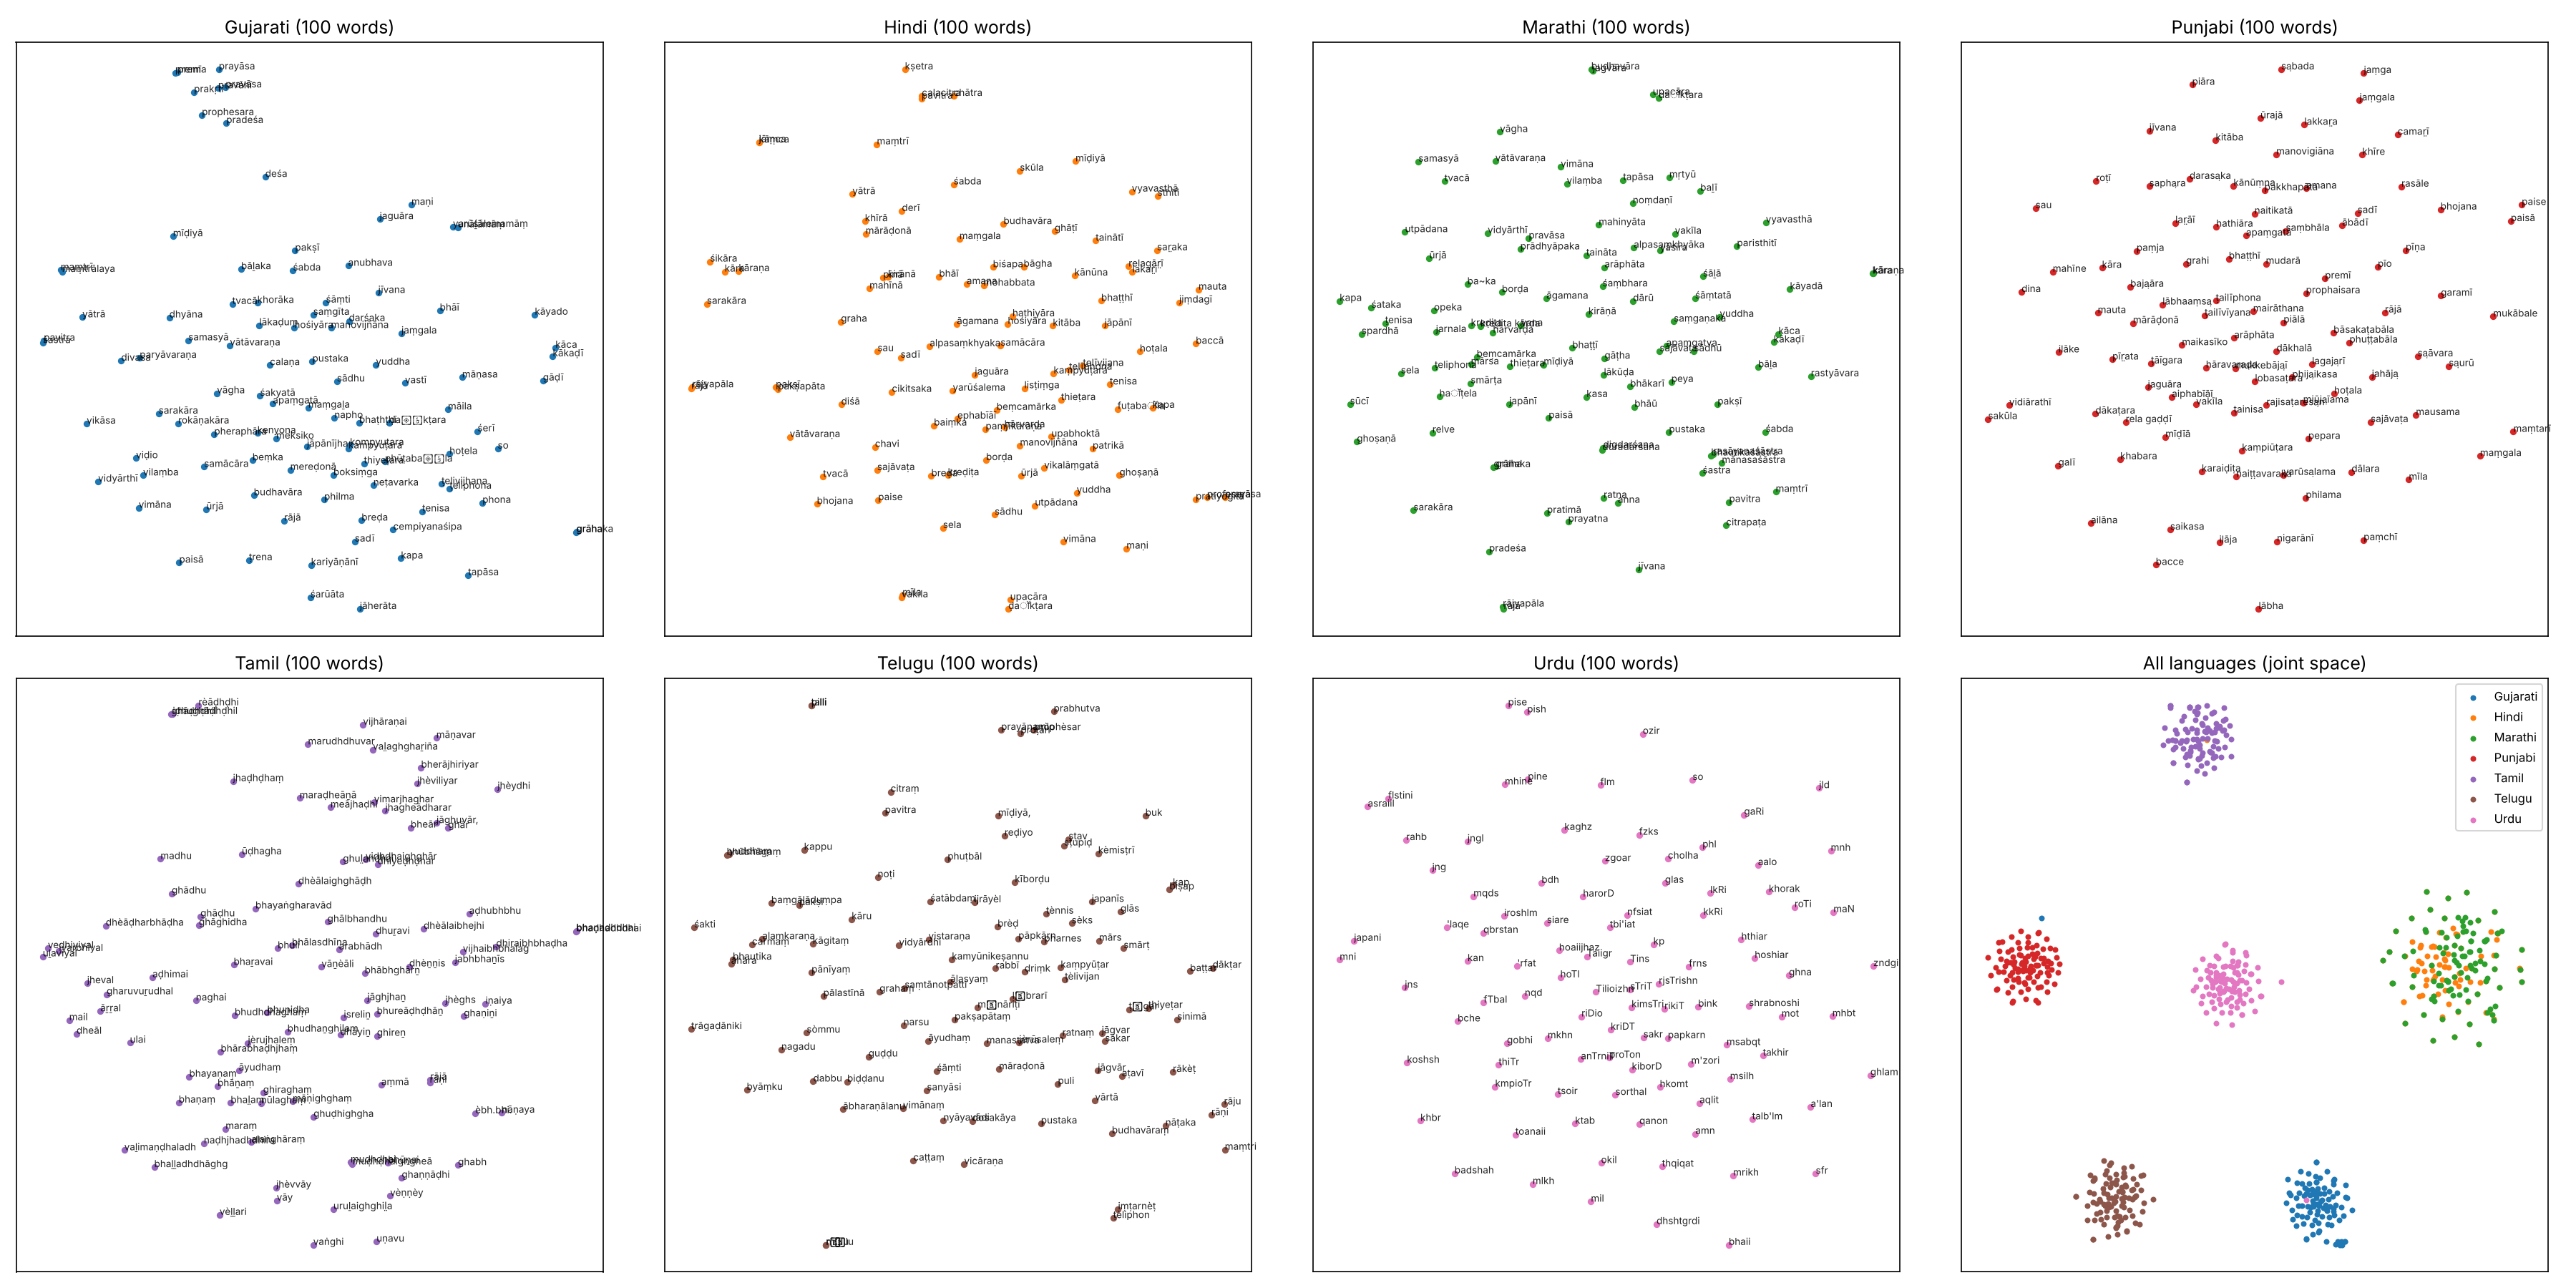
\includegraphics[width=\textwidth]{tsne.png}
\caption{t-SNE projections (perplexity 15 per language, 30 for the joint panel; PCA initialisation; seed 42) of 100 words per language from the final model. Labels are romanised because the plotting library cannot shape Indic scripts.}
\end{figure}

\section{Results}
Table~2 gives the final scores. The macro average is $\rho = 0.240$. Correlations are significant at $p<0.05$ for Gujarati, Hindi, Marathi, Punjabi, Tamil, Urdu; for Telugu they are not, so those estimates should be read with caution. The benchmarks are small (96--235 scored pairs), so each per-language $\rho$ is uncertain: with $n\approx100$ the 95\% confidence interval of a correlation near 0.25 is roughly $\pm0.19$. Differences of a few hundredths between languages or configurations are therefore not meaningful.
\begin{table}[H]\centering\small
\caption{Final model on the public benchmark: Spearman $\rho$ between model cosine similarity and human scores.}
\begin{tabular}{lrrr}\toprule
Language & Pairs (exported) & Pairs with human score & Spearman $\rho$ \\\midrule
Gujarati & 163 & 163 & 0.333 \\
Hindi & 235 & 235 & 0.200 \\
Marathi & 253 & 104 & 0.228 \\
Punjabi & 143 & 143 & 0.297 \\
Tamil & 97 & 96 & 0.239 \\
Telugu & 111 & 111 & 0.174 \\
Urdu & 100 & 100 & 0.209 \\
\midrule
\textbf{Macro average} & 1102 & 952 & \textbf{0.240} \\
\bottomrule\end{tabular}\end{table}

\begin{table}[H]\centering\small
\caption{Vocabulary coverage and OOV statistics of the final model (a word is OOV if any of its tokens is outside the 102k-word training vocabulary). No pair is dropped: OOV words are embedded from character n-grams.}
\begin{tabular}{lrrrrr}\toprule
Language & Unique words & OOV words & Coverage (\%) & Pairs with $\geq$1 OOV & Pairs dropped \\\midrule
Gujarati & 221 & 44 & 80.1 & 47 & 0 \\
Hindi & 318 & 58 & 81.8 & 70 & 0 \\
Marathi & 337 & 64 & 81.0 & 79 & 0 \\
Punjabi & 206 & 33 & 84.0 & 37 & 0 \\
Tamil & 137 & 33 & 75.9 & 36 & 0 \\
Telugu & 160 & 52 & 67.5 & 55 & 0 \\
Urdu & 146 & 20 & 86.3 & 23 & 0 \\
\bottomrule\end{tabular}\end{table}
Coverage ranges from 67.5\% (Telugu) to 86.3\% (Urdu). In total 311 of the 952 scored pairs contain at least one OOV word. The n-gram fallback works reasonably: the mean absolute rank error (percentile rank of the model score minus that of the human score) is 0.309 for pairs with an OOV word against 0.272 for fully in-vocabulary pairs, a small degradation. Telugu has both the lowest coverage and the lowest $\rho$ (0.174). Several Telugu and Tamil benchmark entries are bare stems (e.g.\ {\tel పుస్తక}, {\tam காகித}) that rarely occur on their own in running text. Coverage alone does not explain the ranking, though: Urdu has the best coverage but a mid-range $\rho$.

\section{Experiments}
All experiments train from scratch on IndicCorpV2-5k and are scored with the evaluation of Section~2.5 (Table~4). The numbers were produced with the configurations listed in the notebook (\texttt{EXPERIMENTS}). Setting \texttt{RUN\_EXPERIMENTS=True} reruns them all.
\begin{table}[H]\centering\scriptsize\setlength{\tabcolsep}{3.5pt}
\caption{All experiments (Spearman $\rho$ per language on the public benchmark; time = training seconds on 2 CPU cores). Bold = final model.}
\begin{tabular}{lrrrrrrrrr}\toprule
Configuration & Guj & Hin & Mar & Pan & Tam & Tel & Urd & \textbf{Macro} & Time \\\midrule
E1 PPMI-SVD, win 5 & 0.244 & 0.169 & 0.152 & 0.125 & 0.140 & 0.043 & 0.188 & 0.151 & 41 \\
E2 PPMI-SVD, win 2 & 0.167 & 0.086 & -0.013 & 0.034 & 0.135 & -0.012 & 0.152 & 0.079 & 46 \\
E3 PPMI-SVD, win 8 & 0.252 & 0.215 & 0.135 & 0.158 & 0.137 & 0.092 & 0.188 & 0.168 & 74 \\
E4 PPMI-SVD, win 5, shift log 5 & 0.276 & 0.169 & 0.152 & 0.158 & 0.223 & 0.087 & 0.188 & 0.179 & 60 \\
E5 PPMI-SVD, win 5, rare<20 blended & 0.266 & 0.212 & 0.135 & 0.168 & 0.223 & 0.006 & 0.201 & 0.173 & 58 \\
E6 PPMI-SVD, win 5, p = 0 & 0.216 & 0.198 & 0.206 & 0.193 & 0.179 & 0.065 & 0.125 & 0.169 & 57 \\
E7 FastText SG, 5 ep, sample 1e-4 & 0.072 & -0.080 & 0.123 & 0.164 & 0.121 & -0.061 & -0.095 & 0.035 & 119 \\
E8 E7 on all 24 languages & -0.139 & 0.035 & 0.192 & 0.126 & 0.088 & -0.217 & -0.131 & -0.007 & 416 \\
E9 FastText SG, 20 ep & 0.297 & 0.115 & 0.212 & 0.302 & 0.275 & 0.152 & 0.145 & 0.214 & 556 \\
\textbf{E10 FastText SG, 35 ep} & \textbf{0.334} & \textbf{0.200} & \textbf{0.229} & \textbf{0.298} & \textbf{0.239} & \textbf{0.173} & \textbf{0.209} & \textbf{0.240} & \textbf{1032} \\
E11 FastText CBOW, 35 ep & 0.088 & 0.068 & 0.030 & 0.151 & 0.328 & 0.033 & 0.105 & 0.115 & 417 \\
E12 Skip-gram, no subwords, 20 ep & 0.126 & 0.020 & 0.011 & 0.267 & 0.125 & 0.001 & -0.144 & 0.058 & 405 \\
\bottomrule\end{tabular}\end{table}
\textbf{Training length matters most.} With 5 epochs and aggressive sub-sampling ($10^{-4}$), skip-gram is barely better than chance (E7, 0.035). Moving to sub-sampling $10^{-3}$ with 20 and then 35 epochs raises the macro score to 0.214 (E9) and 0.240 (E10). On a corpus this small, each word occurs only a handful of times per epoch, so many passes are needed.

\textbf{More languages did not help.} Training on all 24 languages under the E7 setting lowered the score (-0.007 vs.\ 0.035) and took 3.5$\times$ longer, so the final model uses only the seven benchmark languages.

\textbf{Count-based baseline.} PPMI-SVD trains in about a minute and reaches 0.179 at best (window 5 with shift $\log 5$). A window of 2 is clearly too narrow for such sparse counts (E2). It stays below FastText skip-gram, especially for Telugu.

\textbf{Skip-gram vs.\ CBOW, and subwords.} With the same 35 epochs CBOW reaches 0.115 (E11), against 0.240 for skip-gram. Removing character n-grams (E12, 20 epochs; OOV words then get a zero vector, i.e.\ cosine 0) gives 0.058 against 0.214 for the matching subword model (E9). This isolates the contribution of the subword representation to both in-vocabulary quality and OOV handling. The best configuration (E10) is the final model.

\section{Analysis}
Tables~5 and~6 list five pairs whose model rank agrees closely with the human rank and five with large disagreements. H-rank and M-rank are percentile ranks within the language.
\begin{table}[H]\centering\scriptsize\setlength{\tabcolsep}{3.5pt}
\caption{Correctly ranked pairs (small gap between human and model percentile rank).}
\begin{tabular}{llllrrrl}\toprule
Lang. & Pair & English gloss & Human & Cosine & H-rank & M-rank & OOV \\\midrule
Hindi & {\dev लाभांश} -- {\dev भुगतान} & \textit{dividend -- payment} & 7.8 & 0.594 & 0.87 & 0.87 & no \\
Punjabi & {\gur ਟਾਈਗਰ} -- {\gur ਜਗੁਆਰ} & \textit{tiger -- jaguar} & 8.375 & 0.780 & 0.94 & 0.94 & yes \\
Marathi & {\dev रत्न} -- {\dev रत्नजडित} & \textit{gem -- gem-studded} & 9.375 & 0.767 & 0.98 & 0.98 & yes \\
Tamil & {\tam மருத்துவர்} -- {\tam செவிலியர்} & \textit{doctor -- nurse} & 7.5 & 0.675 & 0.68 & 0.68 & yes \\
Urdu & \mbox{\urd\beginR ہوٹل\endR} -- \mbox{\urd\beginR بکنگ\endR} & \textit{hotel -- booking} & 9 & 0.656 & 0.88 & 0.87 & no \\
\bottomrule\end{tabular}\end{table}
\begin{table}[H]\centering\scriptsize\setlength{\tabcolsep}{3.5pt}
\caption{Incorrectly ranked pairs (large rank gap).}
\begin{tabular}{llllrrrl}\toprule
Lang. & Pair & English gloss & Human & Cosine & H-rank & M-rank & OOV \\\midrule
Hindi & {\dev पैसे} -- {\dev मुद्रा} & \textit{money -- currency} & 8.6 & 0.314 & 0.98 & 0.06 & no \\
Urdu & \mbox{\urd\beginR زندگی\endR} -- \mbox{\urd\beginR موت\endR} & \textit{life -- death} & 9 & 0.382 & 0.88 & 0.04 & no \\
Marathi & {\dev अराफात} -- {\dev जॅक्सन} & \textit{Arafat -- Jackson} & 0 & 0.650 & 0.03 & 0.94 & yes \\
Telugu & {\tel సన్యాసి} -- {\tel బానిస} & \textit{monk -- slave} & 2 & 0.810 & 0.13 & 0.95 & yes \\
Tamil & {\tam பணம்} -- {\tam நாணய} & \textit{money -- currency (stem)} & 8.625 & 0.367 & 0.85 & 0.01 & yes \\
\bottomrule\end{tabular}\end{table}
\textbf{Where it works.} Topically associated pairs that co-occur in news text are ranked well, e.g.\ \textit{dividend--payment} (Hindi) and \textit{hotel--booking} (Urdu). Subwords help with morphology and loanwords: Marathi \textit{ratna--ratnajaḍita} (gem--gem-studded) contains an OOV word but is ranked almost exactly right, because the compound shares its n-grams with the base noun. The Punjabi pair \textit{tiger--jaguar} (both English loanwords, one OOV) and the Tamil \textit{doctor--nurse} (OOV) are also placed correctly.

\textbf{Where it fails.} (1) \emph{Orthographic neighbours and register}: Hindi \textit{paise} (colloquial ``money'') vs.\ \textit{mudrā} (formal ``currency'') is rated 8.6 by humans but gets one of the lowest model scores. The nearest neighbours of \textit{mudrā} are forms of \textit{muddā} (``issue, topic''), which looks alike in Devanagari and is very frequent in news. Shared n-grams pull \textit{mudrā} towards the wrong word, and its formal ``currency'' sense rarely appears next to the colloquial \textit{paise}. (2) \emph{Antonyms}: Urdu \textit{zindagī--maut} (life--death) is rated 9.0 by annotators, who judged relatedness, while the model gives a low cosine. (3) \emph{Transliterated names}: Marathi \textit{Arafat--Jackson} (human 0) is ranked as highly similar. Both words are OOV and share no n-grams. Each is built from n-grams that occur mostly in foreign names, so unrelated names land in the same ``proper-name'' region. (4) \emph{Sparse contexts}: Telugu \textit{sanyāsi--bānisa} (monk--slave, human 2.0) gets a high cosine even though the two words share no n-grams. \textit{bānisa}'s nearest neighbours are abstract character words (\textit{useless}, \textit{dedication}, \textit{honesty}), and the OOV vector of \textit{sanyāsi} falls in the same region of moral and editorial vocabulary. (5) \emph{Truncated stems}: Tamil \textit{paṇam--nāṇaya} (money--currency) uses the oblique stem \textit{nāṇaya}, which rarely occurs alone, so its OOV vector lies far from \textit{paṇam}.

\section{Discussion}
\textbf{Design choices.} (i) \emph{FastText skip-gram} was chosen because subword sharing is the most direct answer to rich morphology, and it gives OOV vectors without a separate model. Skip-gram also outperformed CBOW and PPMI-SVD here. (ii) \emph{One joint model} over the seven languages is simpler to ship than seven models and loses nothing, because the scripts barely overlap. The overlap that does exist (Hindi/Marathi) is mostly shared loanwords. (iii) \emph{Long training} (35 epochs, light sub-sampling) compensates for the tiny corpus. (iv) \emph{Benchmark-side normalisation} identical to the corpus side avoids spurious OOVs from Unicode variants (nukta, ZWJ). (v) \emph{Int8 storage} keeps the deliverable small without measurable loss.

\textbf{Limitations.} The corpus is very small (0.17--0.36M tokens per language), which caps quality. Many benchmark words occur fewer than 10 times (e.g.\ 72\% of Telugu benchmark tokens). The benchmarks mix similarity with relatedness (antonym pairs rated 9/10), which a distributional model only partly captures. Subword sharing pulls words towards look-alike but unrelated words (\textit{mudrā}/\textit{muddā}), and transliterated names cluster together. The public benchmark is small and was also used to choose among configurations, so the reported numbers may be slightly optimistic for the private test set. I kept the search coarse (12 runs) to limit this. Multi-threaded training is not bit-for-bit deterministic, so retraining gives slightly different numbers; the submitted model reproduces the reported ones exactly. Possible improvements are per-language tuning of epochs and n-gram ranges, morphological segmentation, and longer training.

\subsection*{Disclosure of tools, data and models}
\textbf{Pre-trained models:} none. Every vector is learned from random initialisation. \textbf{Training data:} only IndicCorpV2-5k (\texttt{rony000013/indiccorpV2-5k}). No external corpora. \textbf{Evaluation data:} the Akhtar et al.\ (2017) word-similarity files, used only for evaluation and coarse model selection, never for training. \textbf{Software:} Python 3, gensim 4.4.0 (FastText), NumPy, SciPy (Spearman, sparse matrices), scikit-learn (t-SNE, randomised SVD), pandas and pyarrow (data loading), \texttt{regex} (Unicode tokenisation), Matplotlib (figures), \texttt{indic\_transliteration} (romanised plot labels only), XeLaTeX with Noto fonts (this report). \textbf{AI assistance:} an AI assistant (Claude, Anthropic) was used to help write code and draft this report. All experiments were run and all numbers come from the submitted notebook and logs.

\section*{References}
\small
\begin{enumerate}\setlength{\itemsep}{1pt}
\item S. S. Akhtar, A. Gupta, A. Vajpayee, A. Srivastava, M. Shrivastava. Word Similarity Datasets for Indian Languages: Annotation and Baseline Systems. \textit{Proc. 11th Linguistic Annotation Workshop (LAW)}, ACL, 2017.
\item S. Doddapaneni, R. Aralikatte, G. Ramesh, S. Goyal, M. M. Khapra, A. Kunchukuttan, P. Kumar. Towards Leaving No Indic Language Behind: Building Monolingual Corpora, Benchmark and Models for Indic Languages (IndicCorpV2). \textit{Proc. ACL}, 2023.
\item P. Bojanowski, E. Grave, A. Joulin, T. Mikolov. Enriching Word Vectors with Subword Information. \textit{TACL} 5:135--146, 2017.
\item T. Mikolov, K. Chen, G. Corrado, J. Dean. Efficient Estimation of Word Representations in Vector Space. \textit{ICLR Workshop}, 2013.
\item T. Mikolov, I. Sutskever, K. Chen, G. Corrado, J. Dean. Distributed Representations of Words and Phrases and their Compositionality. \textit{NeurIPS}, 2013.
\item O. Levy, Y. Goldberg, I. Dagan. Improving Distributional Similarity with Lessons Learned from Word Embeddings. \textit{TACL} 3:211--225, 2015.
\item L. van der Maaten, G. Hinton. Visualizing Data using t-SNE. \textit{JMLR} 9:2579--2605, 2008.
\item R. Řehůřek, P. Sojka. Software Framework for Topic Modelling with Large Corpora (gensim). \textit{LREC Workshop on New Challenges for NLP Frameworks}, 2010.
\item Dataset: \url{https://huggingface.co/datasets/rony000013/indiccorpV2-5k}; benchmark: \url{https://github.com/syedsarfarazakhtar/Word-Similarity-Datasets-for-Indian-Languages}.
\end{enumerate}
\end{document}
